\chapter{Research framework}
All fluid surface reconstruction methods described in section \ref{sec:related-work} are based on signed scalar field techniques for surface extraction. Given fluid particle displacement, density, and other SPH information these methods are computing scalar signed field (sometimes referred to as signed distance field (SDF)) values for defined 3D grid vertices domain known as Marching cubes domain. After computation of the SDF values on the grid apply the marching cubes algorithm is applied to calculate surface mesh.\\\
Smoothing algorithms, proposed in this thesis are designed in the way that they can be applied to the reconstruction algorithms with the described infrastructure.


In this work the following methods were implemented for surface reconstruction:
\begin{itemize}
  \item \emph{Muller et. al.} described in \cite{Muller}.
  \item \emph{Zhu-Bridson} method described in \cite{ZhuBridson}.
  \item \emph{Solenthaler} method first introduced in \cite{Solenthaler}.
  \item \emph{Onderik et. al.}, proposed in \cite{OnderikEtAl}.
\end{itemize}
All methods use surface extraction computing SDF and extracting the surface mesh using the MC algorithm. The main difference is the way the SDF is defined (see section \ref{sec:related-work}).



\section{Framework architecture}
To simplify further framework development and testing special care was applied to design the class hierarchy. The class diagram is presented in Figure \ref{fig:class-diagam}.

\begin{figure}[H]
	\begin{center}
		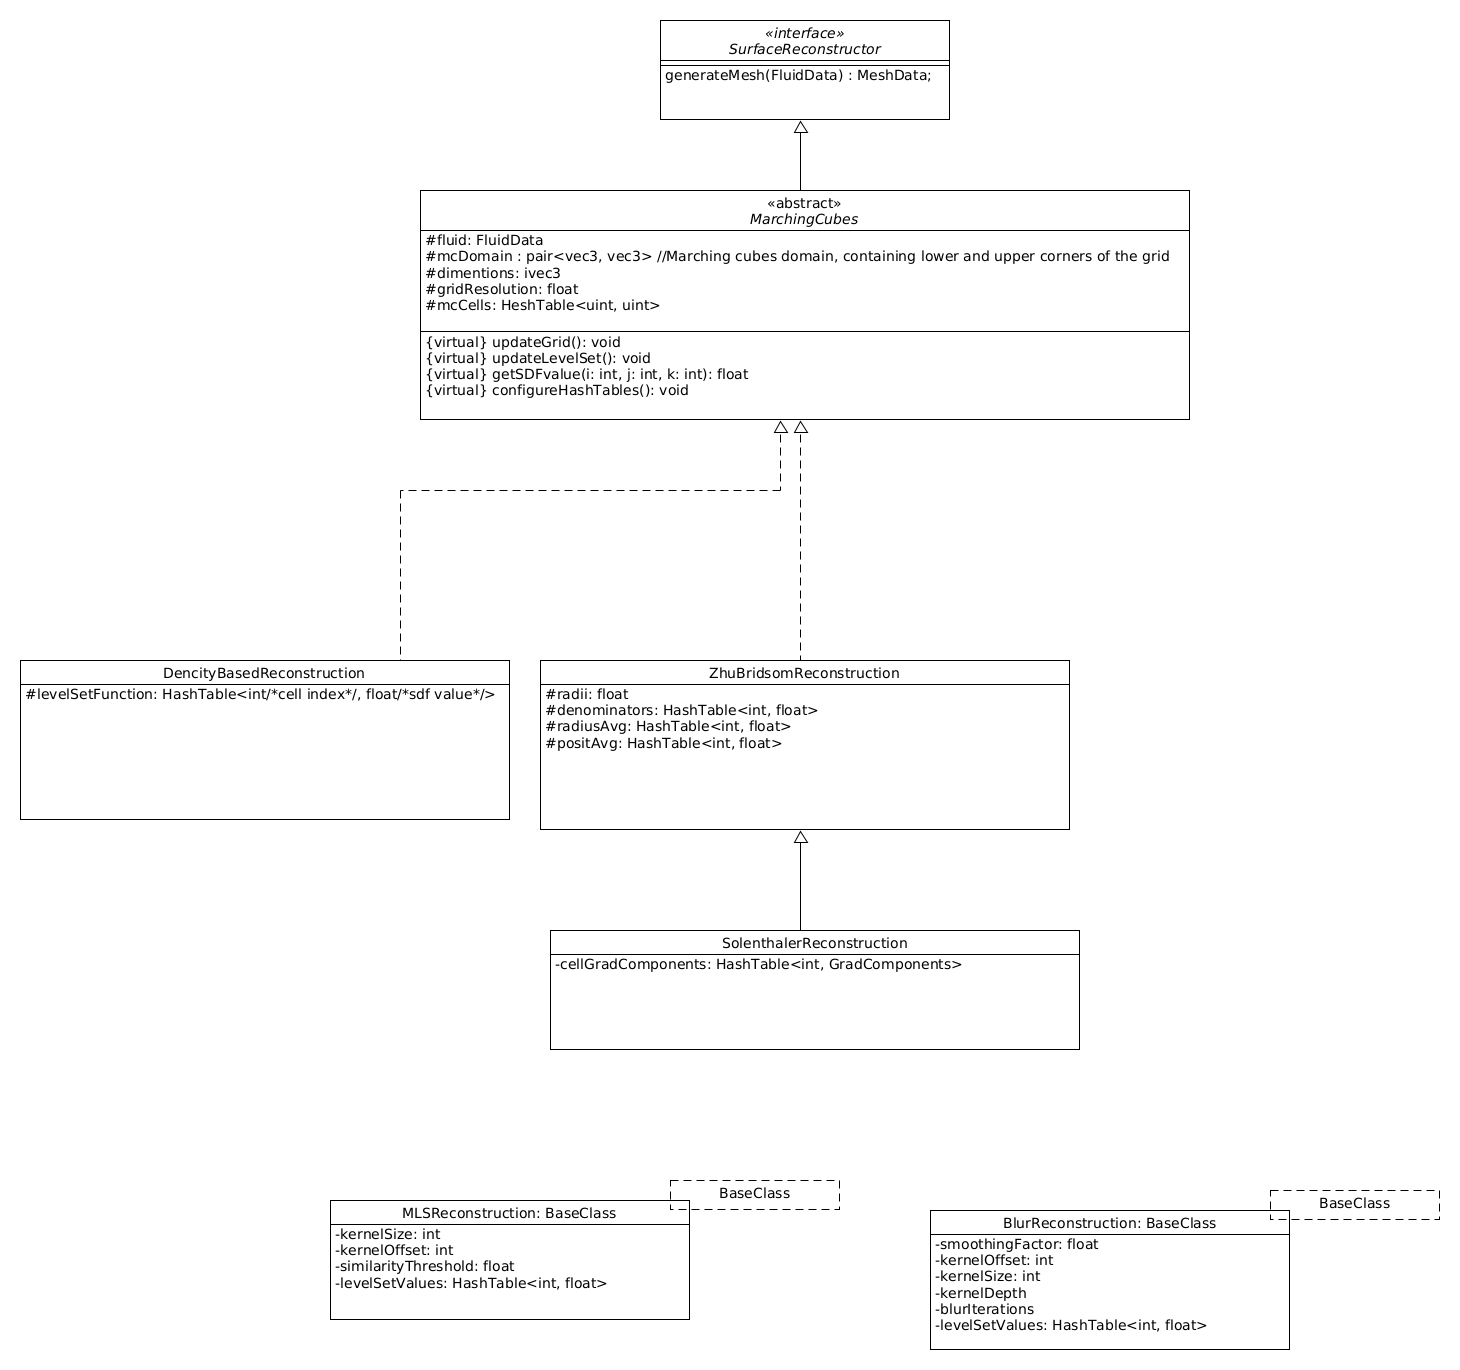
\includegraphics[width=\textwidth]{figures/ClassDiagram.png}
	\end{center}
	\caption{Class diagram, representing inheritance architecture for the surface reconstruction methods}
    \label{fig:class-diagam}
\end{figure}
The base class for all reconstruction methods is \emph{MarchingCubes} class. This class contains common properties for all methods, which exploits the Marching Cubes algorithm. Here \emph{mcDomain} is a pair of two points, representing the domain of marching cubes in 3d space, \emph{dimensions} - is a vector, containing a number of MC grid cells in X, Y, and Z directions, \emph{gridResolution} - the size of each cell (all cells are assumed to be of a uniform size where $width=length=height$), \emph{mcCells} - is a hash table which contains key-value pairs of cell index and a number of SPH fluid particles within its support radius. Each MC cell vertex has its unique integer index, which can be transformed from its position in 3d space. The transformations are extensively explained in \cite{Akinchi}. 
The \emph{MarchingCubes} class has 4 virtual methods, which should be reimplemented inside each subclass:
\begin{itemize}
	\item \emph{computeSurfaceParticles()} - computes color field and detects SPH particles that are resided near the fluid surface.
	\item \emph{configureHashTables()} - inside this method every concrete method performs initial configuration of hash tables, which are used to store SDF.
	\item \emph{updateGrid()} - computes the MC greed domain where calculation of SDF will be performed.
	\item \emph{updateLevelSet()} - calculates SDF values for each MC grid vertex. All smoothing algorithms described here are incorporated in this function and are applied on top of the SDF calculated by underlying method 
\end{itemize}

\emph{MarchingCubes} class re-implements interface method \emph{generateMesh()} composing previously defined functions (see Algorithm \ref{alg:generateMesh}).

\begin{algorithm}
	\scriptsize
	\caption{General overview of the algorithm applied inside each concretisation of MarchingCubes class}
	\label{alg:generateMesh}
	\begin{algorithmic}
		\State $computeSurfaceParticles()$
		\State $configureHashTables()$
		\State $updateGrid()$
		\State $updateLevelSet()$
		\State $mesh \gets computeMesh()$ 
		\State $return\ mesh$
	\end{algorithmic}
\end{algorithm}

\section{Adaptive hash tables for Marching Cubes grid}
As presented in \cite{Akinchi} the computation time for extracting smooth surfaces is mainly influenced by the resolution of the Marching Cubes grid and the smoothing radius R. Achieving high-quality surfaces is possible at the expense of performance. One of the main causes of this issue is computing the scalar field over the volume of the fluid instead of concentrating on the surface area. Thus for performance and memory optimization reasons we decided to apply suggestions, proposed in \cite{Akinchi}.

The first step is to determine the MC grid domain, on which all computation operations will be performed. To perform fluid surface reconstruction it is enough to compute SDF for MC grid cells that are near the fluid surface. To compute these cells next steps are applied:
\begin{itemize}
		\item Compute SPH fluid particles, that are in the nearest neighborhood to the surface of the fluid. To determine surface particles in a preprocessing step, the smoothed color field method \cite{ColorField} is employed.  The smoothed color field value of a particle at position x is computed using Equation \ref{eq:ColorField}.
		\item For each determined particle compute MC grid vertices, that are within the support radius R from each SPH particle, computed in the previous step.
		\item To avoid double layering problem explained in the \cite{Akinchi} additional pass through all SPH particles applied. In this pass for each SPH particle, neighboring MC vertices are queried. If there exists at least one MC grid cell that was identified as a near-surface vertex, the particle is accepted for further processing, otherwise, it is discarded (only for a current frame of the surface reconstruction phase. Modifications are not propagated to the SPH simulation or other reconstruction frames).
\end{itemize}

\begin{equation} \label{eq:ColorField}
	cf_i = \sum_{j\in SPHNeighbors_i}{m_j \cdot \dfrac{W_{ij}}{\rho_j}}
\end{equation}
Where:
\begin{conditions}
	SPHNeighbors_i & set of neighbor fluid particles for particle i\\
	W_{ij} & kernel function\\
	\rho_j & density of particle j\\
\end{conditions}
Detailed instructions sequence described in Algorithm \ref{alg:MC_grid_domain_computation}.
\begin{algorithm}
	\scriptsize
	\caption{Compute MC grid vertices and SPH particles that are going to be processed during computation of the SDF.}
	\label{alg:MC_grid_domain_computation}
	\begin{algorithmic}
		\ForAll{ $particle \in ParticleSet$}
			\State Compute ColorField using Equation \ref{eq:ColorField}
			\If{$ColorField \in ThresholdRange$}
				\State $SurfaceParticleSet \gets SurfaceParticleSet \cup particle$
			\EndIf
		\EndFor

		\ForAll{$particle \in SurfaceParticleSet$}
			\State Compute $Neighbors_i$ of MC vertices within R from  $particle$
			\State $MCGridSurfaceCells \gets MCGridSurfaceCells \cup Neighbors_i$
		\EndFor

		\ForAll{$particle \in ParticleSet$}
			\State Compute $Neighbors_i$ from MCGridSurfaceCells within R from  $particle$
			\If{$Neighbors_i \neq \emptyset$}
				\State $SurfaceParticleSet \gets SurfaceParticleSet \cup particle$
			\EndIf
		\EndFor

		\State $return\ MCGridSurfaceCells, SurfaceParticleSet$
	\end{algorithmic}
\end{algorithm}

As a result the framework is able to perform surface extraction on large scale with up to 13 million SPH particles (see sections \ref{sec:related-work}, \ref{sec:mls} and \ref{sec:blur})
